\documentclass{article}
\usepackage[T1]{fontenc}
\usepackage[utf8]{inputenc}
\usepackage[magyar]{babel}
\usepackage{geometry}
\usepackage{fancyhdr}
\usepackage{hyperref}
\usepackage{graphicx}
\usepackage{listings}
\usepackage{xcolor}
\usepackage{tikz}
\usepackage{pgfplots}
\pgfplotsset{compat=1.18}
\usepackage{pgf-pie}
\usepackage{pdflscape}
\usepackage{float}
\usetikzlibrary{arrows,positioning,shapes.geometric,shapes.misc,shapes.multipart}

\geometry{a4paper, margin=1in}

\title{Flowium Dokumentáció}
\author{py-snake}
\date{\today}

\pagestyle{fancy}
\fancyhf{}
\fancyhead[L]{Flowium Dokumentáció}
\fancyfoot[C]{\thepage}

\hypersetup{
    colorlinks=true,
    linkcolor=blue,
    filecolor=magenta,
    urlcolor=cyan,
}

\definecolor{codegreen}{rgb}{0,0.6,0}
\definecolor{codegray}{rgb}{0.5,0.5,0.5}
\definecolor{codepurple}{rgb}{0.58,0,0.82}
\definecolor{backcolour}{rgb}{0.95,0.95,0.92}

\lstdefinestyle{mystyle}{
    backgroundcolor=\color{backcolour},
    commentstyle=\color{codegreen},
    keywordstyle=\color{magenta},
    numberstyle=\tiny\color{codegray},
    stringstyle=\color{codepurple},
    basicstyle=\footnotesize\ttfamily,
    breakatwhitespace=false,
    breaklines=true,
    captionpos=b,
    keepspaces=true,
    numbers=left,
    numbersep=5pt,
    showspaces=false,
    showstringspaces=false,
    showtabs=false,
    tabsize=2,
    extendedchars=true,
    literate=
        {á}{{\'a}}1 {é}{{\'e}}1 {í}{{\'i}}1 {ó}{{\'o}}1 {ö}{{\"o}}1 {ő}{{\H{o}}}1 {ú}{{\'u}}1 {ü}{{\"u}}1 {ű}{{\H{u}}}1
        {Á}{{\'A}}1 {É}{{\'E}}1 {Í}{{\'I}}1 {Ó}{{\'O}}1 {Ö}{{\"O}}1 {Ő}{{\H{O}}}1 {Ú}{{\'U}}1 {Ü}{{\"U}}1 {Ű}{{\H{U}}}1
}

\lstset{style=mystyle}

\begin{document}

\maketitle

\begin{abstract}
Ez a dokumentum a Flowium projekt részletes dokumentációja. A Flowium fantázianévre hallgató projekt egy olyan forgalomfigyelő és előrejelző rendszer, ami többféle docker konténer szolgáltatására épül. Maga a program Pythonban készült, használ hozzá Dockert és több nyílt forráskódú könyvtárat is, mint például yt-dlp, ffmpeg, opencv2, yolov8. A rendszer képes élő videófolyamot rögzíteni, fel is ismeri, illetve követni tudja a járművek mozgását. Az adatokat sqlite adatbázisban eltárolja, és gépi tanulás segítségével próbálja megjósolni, hogy milyen lesz a forgalom a későbbiekben.
\end{abstract}

\tableofcontents

\newpage

\section{A Projekt Kiindulópontja és Ötlete}

\subsection{Bevezető}
BSc tanulmányaim során mások projektjeit, szakdolgozatát figyelve felkeltette az érdeklődésem az objektum detektálás képeken, valósidejű videón. Ugyan érdeklődésem megvolt a téma iránt, de soha nem volt szükségem ilyen jellegű projektre a hétköznapokban. A féléves feladat kapcsán ötleteltem, átgondoltam hogy lehetne összekötni ezt az évek óta meglévő kíváncsiságot és a tantárgy követelményeit. Egy barátom által fejlesztett rendszerben megláttam a valósidőben tanuló neurális hálózatok szépségét, és a Tanár úr által mondott órai példa, jármű detektálás alapján jött a következő ötlet: járműdetektálás valós időben élő kamera képről és valósidőben tanuló neurális hálózat tanítása forgalmi adatok becslésére, időpont és akár időjárási körülmények figyelembevételével.

A tervem egy forgalom becslő alkalmazás elkészítése, amely egy közúti kamera képe alapján tanul. Sok online, élőben elérhető közterületet vagy közutat figyelő kamerát átnéztem, de legnagyobb bánatomra ezek annyira voltak élők, hogy percenként 1 képet rögzítettek. Jobb esetben 10-15 másodpercenként érkezett egy kép. Ezek a célra egyáltalán nem felelnek meg, ennyi idő alatt számtalan jármű elhaladhat alattuk. Végül az összes magyar kamerás oldal átnézése után eszembe jutott a YouTube élők átnézése mint opció, és találtam is egy 2023 óta folyamatosan közvetítő Bajai kamera képet, amely egy parkra és közútra néz, 1920x1080 pixel felbontással és 30fps képkockasebességgel rendelkezik. Ez a forrás véleményem szerint megfelelő a feladatra. Amennyiben nem sikerül használható minőséget kapni róla, külföldi kamerára vagy rögzített videó fájlra való átállás lesz szükséges.

A következő fejezetekben a technikai megvalósítás lehetséges megközelítéseit vázolom, ami persze előretekintve jó ötletnek tűnik, de a megvalósítás során változhat.

\subsection{Élő kamerakép}
A bevezetőben ismertetett, YouTube-on elérhető Bajai Sugovica-sétányra néző kamera a tervezett videó forrás. Technikai adatai közé tartozik az 1920x1080 pixel képfelbontás és 30fps képkockasebesség. Az adás élő, 7/24 közvetített. A látott kép 3 fő szekcióra osztható: égbolt (időjárási viszonyok, napszak, természeti jellemzők), gyalogos sétány (szerencsés esetben követhető lenne a gyalogos forgalom, de jelenlegi feltételezésem alapján túl apró a kép hozzá), közút (sajnos az út egy részét fák takarják, de egy szakaszon tökéletes rálátás van a közlekedő járművekre). A kamera nappali fényviszonyok mellett kiváló képet közvetít, az éjszaka során az erős kivilágításnak köszönhetően sincs túlságosan sok zaj a képen.

Az élő streamet yt-dlp, ffmpeg és opencv segítségével tudnám betölteni és hasznosítani.

\subsection{Kamerakép előfeldolgozása}
Mint korábban említettem, a kamera nagy területet fog be, ezeket különbözően lehetne hasznosítani. Elsősorban a járművek detektálására szeretnék koncentrálni, ehhez egy körülbelül 800x400 pixel területre kéne koncentrálni.

A hardveres erőforrásaim erősen korlátazottak, GPU egyáltalán nem áll rendelkezésemre, tehát a lehető leghatékonyabban kell elkészíteni a programot. A feldolgozásra vagy laptop processzor (Intel(R) Core(TM) i5-8350U CPU @ 1.70GHz, 4C/8T) vagy bérelt vps dedikált 4 magja (AMD EPYC 9634 84-Core Processor @ 2.20GHz, 4C/4T) áll rendelkezésemre.

A beérkező 1920x1080 képből első lépésként a közutat rögzítő, körülbelül 800x400 pixeles kép kivágását kell megtenni, majd esetlegesen napszaktól, időjárási viszonyoktól függően opencv segítségével hisztogram kiegyenlítést, kontrasztfokozást, zajszűrést végezni. A bejövő 30fps helyett valószínűleg 4-8fps közötti feldolgozási sebesség lesz reális a rendelkezésre álló hardveren, tehát minden 4-7. frame fog feldolgozásra kerülni, a többi eldobásra.

\subsection{Járműdetektálás az előfeldolgozott képeken}
A kamerakép oldalnézetből mutatja a közutat, de még így is látható az elhaladó járművek alakja, mozgása. A detektálásukhoz YOLOv5 vagy YOLOv8 alapú megközelítést tartok reálisnak. Ezzel a módszerrel a tervek szerint felismerhető és követhető lesz a járművek mozgása valósidőben. A detektálás körülményeit, mint dátum, időpont, (időjárási körülmények) egy csv állományban vagy esetleg adatbázisban tárolnám, valamint átadnám a valósidőben tanuló neurális hálónak. A rögzített adatok később jó dataset-ként szolgálhatnának, mivel valós környezetben, több paraméter feljegyzésével lennének tárolva. Ebből később más neurális hálókat is lehetne tanítani, esetleg teljesítményt összehasonlítani. Forgalmat becsülni a jövőre nézve.

A mozgást ugyan lehetne opencv alapokon detektálni, de tartok tőle hogy az oldalnézet, távoli kamerakép miatt nem birkózna meg a feladattal az elvárt pontossággal neurális háló bevetése nélkül.

\subsection{Adatrögzítés, mentés}
A detektált objektumokról készülő feljegyzéseket egyszerű csv szöveges állományban is lehetne tárolni, de ha hosszútávú üzemeltetés a cél, jobb lenne valamilyen adatbázist használni, például egyszerű helyi SQLite alapú tárolást. Ez a megközelítés jelentősen gyorsítaná nagy mennyiségű adat tárolását, és nem járna nagy többlet erőforrás igénnyel. A feldolgozás jelentősen gyorsul, lekérdezések, keresések, statisztikák, exportálás, biztonsági mentés könnyedén végezhető.

A tárolni kívánt adatmezőket a későbbiekben szeretném pontosan meghatározni attól függően, hogy milyen adatok lesznek elérhetők (például az időbélyegen kívül esetleg autó típus méret alapján, ideiglenes egyedi azonosító a járműre, konfidencia). Amennyiben időjárásadatok és esetleg más, a forgalmat befolyásoló tényezők tárolása bevezetésre kerülne, további adatmezőket kell felvenni.

\subsection{Valós idejű tanulás}
A terv egy online tanuló rendszer elkészítése, amely a beérkező adatokat feldolgozva folyamatosan képes a tanulásra. A megvalósításhoz a River python csomag illeszkedne, mivel online tanuló algoritmusok vannak benne implementálva. A módszer előnye, hogy nem lenne időszakosan kimagasló erőforrásigénye, hanem egy folyamatos egyenletes terhelést jelentene a rendszer számára. Ezzel a megközelítéssel nem lenne szükség a régi adatok újra tanulására, hanem a modell folyamatosan frissítésre kerülne.

\subsection{Kiegészítő adatok, például időjárás és környezeti tényezők}
A forgalmat és a járműdetektálás sikerességét egyaránt befolyásolhatják az időjárási tényezők, ezért véleményem szerint érdemes lenne feljegyezni ezeket az adatokat is. Az időjárási viszonyok hatást gyakorolhatnak a forgalom sűrűségére, így ezek rögzítésével lehetne elemezni az összefüggéseket, és esetleg pontosabb becslést adni a felépített modellel. A rossz látási viszonyok a járműdetektálást is negatívan befolyásolhatják, mivel esős viharos időben jelentősen romlik a kamera által rögzített kép. Ekkor elképzelhető lehet, hogy ugyan a valóságban megnő a forgalom, de a rossz képminőség miatt csak a járművek töredéke lesz feljegyezve.

Az időjárásadatok forrása lehetne maga a kamerakép, valamilyen módon felismerni a környezeti tényezőket valós időben. Ez nagy erőforrásigénnyel járna és korlátozottan lehetne eljárni. Ezzel ellentétes megközelítés egy időjárás API használata, vagy időjárás weboldalról legyűjtött adatok használata. Ennek előnye, hogy jóval kevesebb erőforrásra van szükség hozzá, több környezeti jellemzőhöz tényszerűen hozzá lehet férni (hőmérséklet, páratartalom, eső vagy napsütés, napfelkelte, napnyugta, szélerősség), viszont hátránya, hogy bizonyos esetekben pontatlan lehet. Pontatlanságot okozhat, ha az online előrejelzés szerint az adott időszakban esőzés van a területen, ám a kamera képe szerint csak felhős az idő, de a valóságban nem esik eső. Ennek kiküszöbölésére hibrid megközelítést lehetne alkalmazni, de ez jelenleg túlmutat a projekt keretein.

A rögzített időjárási adatokkal elemehetővé válik a forgalmi minta és az időjárás összefüggése, vagy a detektálási hiba alakulása nem várt időjárási körülmények közt.

\subsection{Futtatási környezet, rendszerek összekapcsolása}
A projekt megvalósítása Python programozási nyelven tervezett, különböző Python könyvtárak felhasználásával. Az egységbe csomagolás, könnyű telepítés és hordozhatóság érdekében a teljes rendszert szerepkörök alapján felbontva, docker alapú konténerekbe szervezve, API alapú kommunikációval tervezem megvalósítani. A tervezett szerepkörök körülbelül megfelelnek a felsorolt pontoknak: élő kamerakép fogadása (yt-dlp), kép előfeldolgozása (ffmpeg, opencv), járműdetektálás (YOLO), adatrögzítés (SQL vagy SQLite), online tanulás (River), kiegészítő szolgáltatások, például időjárás API.

\subsection{Használni tervezett rendszerek}

\begin{table}[h]
\centering
\begin{tabular}{|l|l|p{7cm}|}
\hline
\textbf{Kategória} & \textbf{Technológia} & \textbf{Felhasználás} \\
\hline
Programozási nyelv & Python & Fejlesztési környezet \\
Videó stream & yt-dlp & YouTube stream letöltése \\
Videó feldolgozás & Ffmpeg & Videó feldolgozása \\
Gépi látás & OpenCV & Videó és kép feldolgozása \\
Objektum detektálás & YOLOv5 vagy YOLOv8 & Járműdetektálás és követés \\
Adatbázis & SQLite & Adattárolás \\
Online tanulás & River & Valós idejű modell létrehozása \\
Adatmanipuláció & Pandas & Adatfeldolgozás \\
Adatmanipuláció & NumPy & Adatfeldolgozás \\
Webkliens & Requests & API kommunikáció \\
Webkliens & curl & Web és API kommunikáció \\
Vizualizáció & Matplotlib & Grafikonok \\
Vizualizáció & Seaborn & Statisztikai ábrák \\
API keretrendszer & FastAPI & REST API végpontok \\
Machine learning & Scikit-learn & Modellek \\
Konténerizáció & Docker & Környezetek futtatása \\
Verziókezelés & Git & Fejlesztés követése \\
\hline
\end{tabular}
\caption{A projekt megvalósításához tervezett technológiai stack}
\end{table}

\subsection{Mintaképek}
Nappali és éjszakai mintakép. Jól látható, hogy szép időjárás és megfelelő fényviszonyok közt elég jó a képminőség, a feladatnak megfelelő lesz a forrás. Mintakép a járműdetektálás szempontjából releváns területről. Az eltérő időpontok kissé eltérő színvilágú képeket eredményeznek.

\begin{figure}[H]
    \centering
    \includegraphics[width=\linewidth]{image/kep_1.png}
    \caption{Mintakép 1}
    \label{fig:kep1}
\end{figure}

\begin{figure}[H]
    \centering
    \includegraphics[width=\linewidth]{image/kep_2.png}
    \caption{Mintakép 2}
    \label{fig:kep2}
\end{figure}

\begin{figure}[H]
    \centering
    \includegraphics[width=\linewidth]{image/kep_3.png}
    \caption{Mintakép 3}
    \label{fig:kep3}
\end{figure}

\newpage

\section{Rendszerarchitektúra}
A Flowium projekt mikroszolgáltatás elven épül fel. Az egyes szolgáltatások Docker konténerekben futnak, ezek indítását és kezelését pedig a Docker Compose végzi. Ez a megoldás azért előnyös, mert a rendszer így jó modularitással rendelkezik, könnyen bővíthető vagy karbantartható, és a skálázhatóság is biztosított.

\subsection{Docker Compose áttekintés}
A rendszer működésének központja a \texttt{docker-compose.yml} fájl, amelyben pontosan szerepel, hogy melyik szolgáltatás mit csinál, és hogyan kapcsolódnak egymáshoz. Összesen hét fő szolgáltatás tartozik a rendszerhez, ezek egy közös, \texttt{flowium-network} nevű Docker hálózaton keresztül kommunikálnak. Az adatok tárolásához Docker volume-ok, vagyis virtuális kötetek kerülnek felhasználásra.

\begin{itemize}
    \item \textbf{stream-capture:} Ez a szolgáltatás a YouTube-ról érkező élő videófolyam fogadásáért felel.
    \item \textbf{preprocessing:} Itt zajlik a bejövő videó képkockáinak előfeldolgozása.
    \item \textbf{yolo-detector:} Ebben a lépésben történik a járművek felismerése az előfeldolgozott képeken.
    \item \textbf{data-manager:} Ez a modul tartalmazza az adatbázist és tárolja az összes begyűjtött adatot.
    \item \textbf{online-learner:} Itt valósul meg a gépi tanulás, ami a forgalmi minták előrejelzésére szolgál.
    \item \textbf{weather-service:} Ez a szolgáltatás szerzi be az aktuális időjárási adatokat.
    \item \textbf{web-ui:} A rendszerhez tartozó webes felület, amelyen keresztül minden funkció elérhető és követhető.
\end{itemize}

\newpage
\begin{landscape}
\thispagestyle{empty} % Optional: removes header/footer on this page
\begin{figure}[h]
	    \centering
    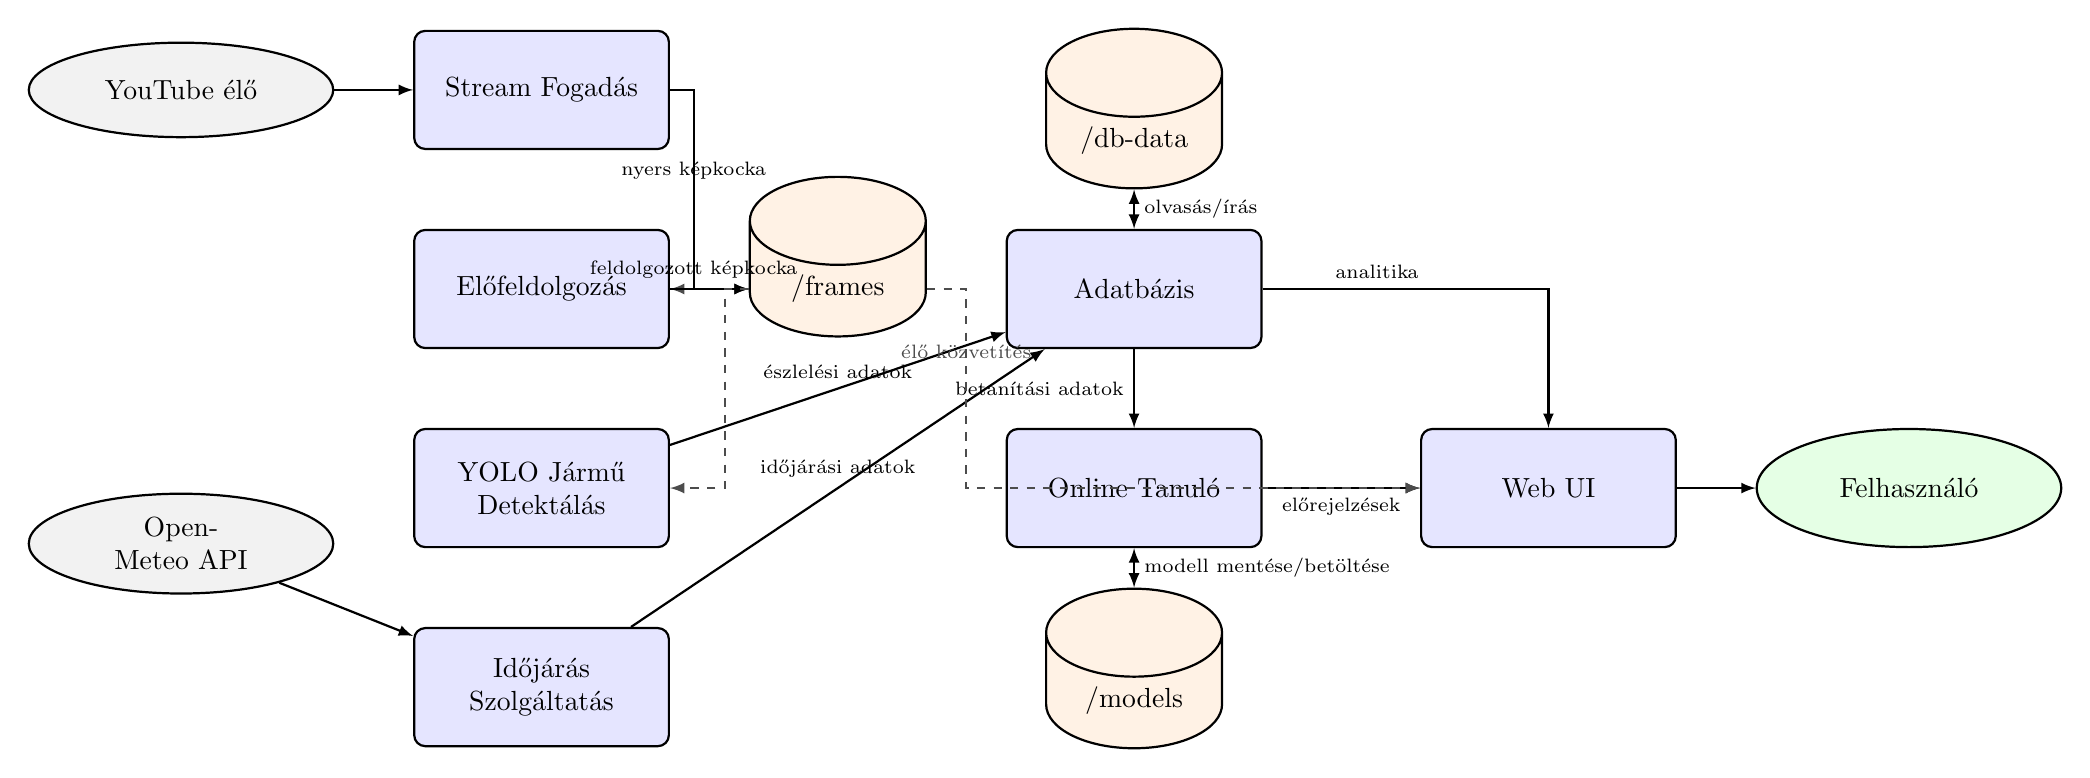
\begin{tikzpicture}[
        node distance=1.5cm and 1cm,
        service/.style={rectangle, draw, thick, rounded corners, fill=blue!10, text centered, minimum height=1.5cm, text width=3cm},
        ext_source/.style={ellipse, draw, thick, fill=gray!10, text centered, minimum height=1.2cm, text width=2.5cm},
        storage/.style={cylinder, draw, thick, shape border rotate=90, fill=orange!10, text centered, minimum height=1.2cm, text width=2cm, aspect=0.5},
        user/.style={ellipse, draw, thick, fill=green!10, minimum height=1.5cm, text width=2.5cm, text centered},
        arrow/.style={->, >=latex, thick},
        data_arrow/.style={->, >=latex, dashed, thick, color=black!70}
    ]

    % External Sources
    \node[ext_source] (youtube) {YouTube élő};
    \node[ext_source, below=4.5cm of youtube] (openmeteo) {Open-Meteo API};

    % First column of services
    \node[service, right=of youtube] (stream) {Stream Fogadás};
    \node[service, below=1cm of stream] (preproc) {Előfeldolgozás};
    \node[service, below=1cm of preproc] (yolo) {YOLO Jármű Detektálás};
    \node[service, below=1cm of yolo] (weather) {Időjárás Szolgáltatás};

    % Shared Volumes
    \node[storage, right=of preproc] (frames) {/frames};
    
    % Second column of services (Data/ML)
    \node[service, right=of frames] (datamgr) {Adatbázis};
    \node[service, below=1cm of datamgr] (learner) {Online Tanuló};

    % More Shared Volumes
    \node[storage, above=0.5cm of datamgr] (dbdata) {/db-data};
    \node[storage, below=0.5cm of learner] (models) {/models};

    % Third column (UI)
    \node[service, right=2cm of learner] (webui) {Web UI};
    
    % User
    \node[user, right=of webui] (user) {Felhasználó};

    % Arrows - Data Flow
    \draw[arrow] (youtube) -- (stream);
    \draw[arrow] (openmeteo) -- (weather);

    \draw[arrow] (stream.east) -- ++(0.3,0) |- node[pos=0.25, above, font=\scriptsize] {nyers képkocka} (frames.west);
    \draw[data_arrow] (frames.west) -| ++(-0.3,0) |- (preproc.east);
    \draw[arrow] (preproc.east) -- ++(0.3,0) |- node[pos=0.25, above, font=\scriptsize] {feldolgozott képkocka} (frames.west);
    \draw[data_arrow] (frames.west) -| ++(-0.3,0) |- (yolo.east);
    
    \draw[arrow] (yolo) -- node[above, font=\scriptsize] {észlelési adatok} (datamgr);
    \draw[arrow] (weather) -- node[above, font=\scriptsize] {időjárási adatok} (datamgr);

    \draw[arrow] (datamgr) -- (learner) node[midway, left, font=\scriptsize] {betanítási adatok};
    \draw[arrow, <->] (datamgr.north) -- (dbdata.south) node[midway, right, font=\scriptsize] {olvasás/írás};
    \draw[arrow, <->] (learner.south) -- (models.north) node[midway, right, font=\scriptsize] {modell mentése/betöltése};

    % Arrows - UI and User
    \draw[arrow] (learner) -- (webui) node[midway, below, font=\scriptsize] {előrejelzések};
    \draw[arrow] (datamgr) -| (webui) node[pos=0.2, above, font=\scriptsize] {analitika};
    \draw[data_arrow] (frames.east) -| ++(0.5,0) |- (webui.west) node[pos=0.2, above, font=\scriptsize] {élő közvetítés};
    
    \draw[arrow] (webui) -- (user);

    \end{tikzpicture}
    \caption{Részletes Flowium Rendszerarchitektúra, amely bemutatja a szolgáltatásokat, az adatmennyiségeket és az adatfolyamot.}
    \label{fig:flowium-architecture-detailed}
\end{figure}
\end{landscape}
\newpage

\section{Alapvető algoritmusok}
Ebben a szakaszban bemutatásra kerülnek azok a kulcsfontosságú algoritmusok, amelyek a rendszer működését biztosítják.

\subsection{Járműkövető (\texttt{tracker.py})}
A járműkövető komponens alapvető szerepet tölt be a pontos járműszámok meghatározásában, illetve az adatredundancia elkerülésében. A megvalósítás során egy úgynevezett mohó illesztési algoritmus alkalmazása történik, amely az Intersection over Union (IoU) és a centroid távolság együttes pontszámán alapul.

\begin{itemize}
    \item \textbf{Illesztés:} Minden egyes új képkockához a rendszer minden létező nyomvonalhoz kiszámít egy illesztési pontszámot az újonnan észlelt objektumokra vonatkozóan. Az algoritmus az IoU értéket (ami a térbeli átfedést méri) és a normalizált centroid távolságot (ami a közelséget reprezentálja) kombinálja. Ezáltal lehetővé válik a gyorsan mozgó objektumok hatékony követése.
    \item \textbf{Mohó hozzárendelés:} Az illesztések a pontszámok alapján kerülnek sorba rendezésre, és mindig a legjobb pontszámú párok kerülnek először hozzárendelésre. Ez a módszer gyors és hatékony alternatívát nyújt a bonyolultabb, optimális hozzárendelési algoritmusokkal szemben.
    \item \textbf{Nyomvonal életciklusa:}
    \begin{itemize}
        \item \textbf{Létrehozás:} Minden olyan észlelés, amelyhez nem tartozik illesztett nyomvonal, új nyomvonalat hoz létre.
        \item \textbf{Frissítés:} Ha illesztés történik, az adott nyomvonal pozíciója frissítésre kerül, és a \texttt{hits} számláló értéke növekszik.
        \item \textbf{Törlés:} Azok a nyomvonalak, amelyeket a \texttt{max\_age} paraméterben meghatározott számú képkockán keresztül nem észlel a rendszer, törlésre kerülnek.
    \end{itemize}
    \item \textbf{Megerősítés és hatékonyság:} Egy nyomvonal csak akkor tekinthető megerősítettnek, ha azt legalább \texttt{min\_hits} képkockán keresztül folyamatosan észleli a rendszer. A megoldás lényege, hogy a jármű adatai csak akkor kerülnek egyszer az adatbázisba, amikor a nyomvonal megerősítetté válik. Ezt a folyamatot a nyomvonal adataiban található \texttt{stored} jelző, valamint a \texttt{get\_confirmed\_new\_tracks} metódus kezeli, így az adatbázisba történő írások száma jelentősen csökkenthető.
\end{itemize}

\subsection{Atomi írási mechanizmus (\texttt{stream-capture})}
Ebben a részben bemutatásra kerül, hogy a \texttt{stream-capture} és a \texttt{preprocessing} szolgáltatások hogyan alkalmaznak atomi írási mechanizmust annak érdekében, hogy az alsóbb rétegbeli szolgáltatások ne olvassanak be részben megírt vagy sérült képfájlokat.

A projekt készítése közben felmerült a probléma, hogy az egyik konténer által még csak részlegesen mentett képfájlokat próbált beolvasni egy másik konténer és emiatt hibás adatok készültek.

\begin{enumerate}
    \item Először egy folyamat (például az \texttt{ffmpeg}) egy ideiglenes fájlba írja a képadatokat (\texttt{latest\_writing.jpg} néven).
    \item Egy külön szál folyamatosan figyeli ezt az ideiglenes fájlt, és ellenőrzi annak módosítási idejét, illetve méretét.
    \item Amint a fájl egy rövid ideig stabilan változatlan marad, az írás befejezettnek minősül.
    \item Ezt követően a figyelő szál egy atomi \texttt{os.rename} művelettel átnevezi az ideiglenes fájlt a végleges helyre (például \texttt{latest.jpg}-ra). Ezután már használhatóvá válik a teljes fájl.
\end{enumerate}

\subsection{Adaptív előfeldolgozás}
Ebben a részben bemutatásra kerül, hogy a \texttt{preprocessing} szolgáltatás hogyan alkalmaz adaptív eljárásokat a képek optimalizálására, amely különösen fontos a YOLO észlelő számára eltérő fényviszonyok mellett.

\begin{itemize}
    \item \textbf{Fényerő észlelése:} A képek először HSV színtérre kerülnek átalakításra. Ezután a V (érték/fényerő) csatorna átlagos értéke kerül kiszámításra annak eldöntésére, hogy a jelenet nappali vagy éjszakai.
    \item \textbf{Éjszakai javítás:} Amennyiben sötét jelenetről van szó, a rendszer gamma korrekciót alkalmaz a fényerő növelése érdekében, majd CLAHE (kontrasztkorlátozott adaptív hisztogramkiegyenlítés) kerül felhasználásra magas klipkorláttal, így a helyi kontraszt is javításra kerül, és előtérbe kerülnek az árnyékos részek részletei.
    \item \textbf{Nappali javítás:} Világos jelenetek esetén enyhébb CLAHE művelet zajlik le, amely segíti a kontraszt javítását, ugyanakkor elkerülhető a túlexponálás.
    \item \textbf{Háttérkivonás:} A szolgáltatás lehetőséget biztosít az OpenCV \texttt{createBackgroundSubtractorMOG2} funkciójának alkalmazására, amely során a rendszer statikus háttér statisztikai modelljét hozza létre. Amennyiben ez a funkció engedélyezve van, a nem mozgó objektumok (például fák, oszlopok, épületek) eltávolításra kerülnek a képkockákból, így a járművek izolálhatók és kevesebb zaj jut el az észlelőhöz. A funkció jó, nappali fényviszonyok mellett hatékonynak bizonyult, de sötétedéskor már nem nyújtotta a megfelelő teljesítményt. Az autók a gyors mozgásuk miatt kissé elmosódva, a gyenge fény miatt pedig homályosan látszódtak a funkció használata mellett.
\end{itemize}

\subsection{Online tanulási folyamat}
Ebben a részben bemutatásra kerül, hogy az \texttt{online-learner} szolgáltatás miként alkalmazza a \texttt{river} könyvtárat egy folyamatosan tanuló gépi tanulási modell kialakítására.

\begin{enumerate}
    \item \textbf{Folyamat:} A modell egy \texttt{river.compose.Pipeline} objektum formájában valósul meg, amely két fő lépést kapcsol össze.
    \item \textbf{Standard skálázó:} Az első lépésben a \texttt{preprocessing.StandardScaler} működése során a bemeneti jellemzők (például idő, hőmérséklet) normalizálása történik meg az átlag kivonásával és egységnyi szórásra való skálázással. A \texttt{river} skálázó folyamatosan frissíti ezeket a statisztikákat az új adatok beérkezésekor.
    \item \textbf{Lineáris regresszió:} A második lépésben a \texttt{linear\_model.LinearRegression} használata történik. Ez a modell a skálázott jellemzőkhöz tartozó súlyokat tanulja meg a járműszámok előrejelzése céljából. A súlyok frissítése minden egyes új adatpont esetén az online optimalizálási algoritmusok alkalmazásával valósul meg.
    \item \textbf{Folyamatos betanítás:} Egy háttérfolyamat rendszeresen lekéri az \texttt{data-manager} szolgáltatástól a legfrissebb összesített adatokat, és ezeket folyamatosan betáplálja a modellbe. Ezáltal biztosított, hogy a modell képes legyen alkalmazkodni az újonnan megjelenő forgalmi mintákhoz.
\end{enumerate}

\section{Szolgáltatások}

\subsection{Stream Capture (\texttt{stream-capture})}

\subsubsection{Cél}
Ebben a részben bemutatásra kerül a \texttt{stream-capture} szolgáltatás fő feladata, amely az élő videófolyam fogadását és a képkockák megosztott kötetre történő írását foglalja magában.

\subsubsection{Belső logika}
A szolgáltatás működése az alábbi lépésekben foglalható össze:

\begin{enumerate}
    \item \textbf{Élő videó forrás:} A rendszer a YouTube élő közvetítését használja adatforrásként, amelynek címe a \texttt{YOUTUBE\_URL} környezeti változóban kerül megadásra.
    \item \textbf{Képkocka rögzítése:} A képkockák folyamatos rögzítését az \texttt{ffmpeg} és \texttt{cv2} könyvtárak segítségével végzi, amelyek lehetővé teszik a stream megnyitását és a képkockák kinyerését.
    \item \textbf{Proxy:} A YouTube az adatközponti \texttt{datacenter} IP-ket általában bot-nak jelöli, ezért szükséges \texttt{http proxy} és bejelentkezett Google fiókból kinyert \texttt{cookie-k} használata.
    \item \textbf{Atomi írás:} Az elkészült képkockákat a rendszer atomi írási eljárással menti a \texttt{/frames} megosztott kötetre. Ennek célja, hogy a \texttt{preprocessing} szolgáltatás mindig épségben lévő, teljes képkockákat tudjon beolvasni.
    \item \textbf{Sebesség korlátozás:} A képkockák rögzítési gyakoriságát az \texttt{FPS} környezeti változó szabályozza. Mivel csak CPU-val rendelkező, GPU nélküli gép állt rendelkezésre a megvalósításhoz, tesztek után 5 FPS került meghatározásra felső korlátként, így még lépést tud tartani a CPU a feldolgozással.
\end{enumerate}

\subsubsection{Függőségek}
\begin{itemize}
    \item \textbf{Bemenet:} Élő videófolyam a YouTube csatornáról.
    \item \textbf{Kimenet:} Képkockafájlok a \texttt{/frames} megosztott kötetre.
    \item \textbf{Szolgáltatás függőségek:} Ennél a szolgáltatásnál közvetlen szolgáltatás-függőség nem jelenik meg.
\end{itemize}

\subsubsection{Konfiguráció}
Az alábbi környezeti változók alkalmazásával történik a szolgáltatás beállítása:

\begin{lstlisting}[language=bash, title=Environment Variables]
# A YouTube élő közvetítésének URL-je.
YOUTUBE_URL

# Frames per second (FPS) korlát. Alapértelmezetten: 5
FPS
\end{lstlisting}

\subsection{Preprocessing (\texttt{preprocessing})}

\subsubsection{Cél}
Ebben a részben bemutatásra kerül a \texttt{preprocessing} szolgáltatás célja, amely a nyers képkockák fogadását, azok adaptív javítását és végül a képkockák továbbítását végzi a \texttt{yolo-detector} részére.

\subsubsection{Belső logika}
A szolgáltatás működése az alábbi lépésekben összegezhető:

\begin{enumerate}
    \item \textbf{Képkocka olvasás:} A rendszer folyamatosan beolvassa a legfrissebb képkockát a \texttt{/frames} megosztott kötetről.
    \item \textbf{Adaptív javítás:} Az adaptív előfeldolgozási algoritmus kerül alkalmazásra minden képkockán, hogy az aktuális fényviszonyokhoz igazítsa a képet.
    \item \textbf{Képkocka továbbítás:} Az előfeldolgozott képkockák továbbítása a \texttt{yolo-detector} szolgáltatás felé történik, HTTP POST kérések segítségével.
    \item \textbf{API:} A szolgáltatás egy egyszerű HTTP API-t is kínál, amely lehetővé teszi a konfiguráció futásidőben történő módosítását.
\end{enumerate}

\subsubsection{Függőségek}
\begin{itemize}
    \item \textbf{Bemenet:} Képkockafájlok a \texttt{/frames} megosztott kötetről.
    \item \textbf{Kimenet:} Feldolgozott képkockák a \texttt{yolo-detector} szolgáltatás felé.
    \item \textbf{Szolgáltatásfüggőségek:} Közvetlenül a \texttt{yolo-detector} szolgáltatáshoz kapcsolódik.
\end{itemize}

\subsubsection{Konfiguráció}
A szolgáltatás az alábbi környezeti változóval konfigurálható:

\begin{lstlisting}[language=bash, title=Environment Variables]
# A yolo-detector szolgáltatás URL-je. Alapértelmezett: http://yolo-detector:8000
YOLO_DETECTOR_URL
\end{lstlisting}

\subsection{YOLO Detector (\texttt{yolo-detector})}

\subsubsection{Cél}
Ebben a részben kerül bemutatásra a \texttt{yolo-detector} szolgáltatás fő feladata, amely a járművek észlelését végzi a beérkező képkockákon, illetve a nyomvonalak kezelését is ellátja a \texttt{tracker.py} segítségével.

\subsubsection{Belső logika}
A szolgáltatás működése az alábbi lépésekben foglalható össze:

\begin{enumerate}
    \item \textbf{YOLO modell:} A rendszer a YOLOv8 modellt használja arra, hogy észlelje a különböző járműtípusokat (autókat, teherautókat, buszokat, motorokat) az egyes képkockákon.
    \item \textbf{Nyomvonal kezelés:} Minden észlelt objektum információja átadásra kerül a \texttt{tracker.py} járműkövetőnek, amely a járművek mozgásának folyamatos követését végzi.
    \item \textbf{Adatküldés:} A követő által megerősített új járművekről (például észlelési adatok, járműszám) szóló információk HTTP POST kéréseken keresztül jutnak el a \texttt{data-manager} adatbázis szolgáltatáshoz.
    \item \textbf{Képkocka mentés:} A szolgáltatás elmenti a legfrissebb, észlelésekkel és nyomvonalakkal ellátott képkockát a \texttt{/frames} megosztott kötetre, hogy a \texttt{web-ui} számára elérhető legyen az élő nézethez.
\end{enumerate}

\subsubsection{Függőségek}
\begin{itemize}
    \item \textbf{Bemenet:} Feldolgozott képkockák a \texttt{preprocessing} szolgáltatástól.
    \item \textbf{Kimenet:} Észlelési adatok a \texttt{data-manager} szolgáltatás felé.
    \item \textbf{Szolgáltatásfüggőségek:} Közvetlen kapcsolatban áll a \texttt{data-manager} szolgáltatással.
\end{itemize}

\subsubsection{Konfiguráció}
A szolgáltatás működése az alábbi környezeti változók segítségével testreszabható:

\begin{lstlisting}[language=bash, title=Environment Variables]
# A data-manager szolgáltatás URL-je. Alapértelmezett: http://data-manager:8000
DATA_MANAGER_URL

# YOLO detektálás bizalmi küszöbértéke. Alapértelmezett: 0.5
CONFIDENCE_THRESHOLD

# Egy nyomvonal maximális kora (képkockában), mielőtt törlésre kerülne. Alapértelmezett: 30
MAX_AGE

# Egy nyomvonal megerősítéséhez szükséges minimális találatok száma. Alapértelmezett: 3
MIN_HITS
\end{lstlisting}

\subsection{Data Manager (\texttt{data-manager})}

\subsubsection{Cél}
Ebben a részben kerül bemutatásra a \texttt{data-manager} szolgáltatás célja. Ez a rendszer központi adatbázisaként működik, mely képes fogadni, eltárolni és aggregálni az összes jármű- és időjárási adatot.

\subsubsection{Belső logika}
A szolgáltatás működése az alábbi pontokban foglalható össze:

\begin{enumerate}
    \item \textbf{Adatbázis:} A rendszer egy SQLite adatbázist használ, amely a \texttt{/db-data} megosztott köteten kerül tárolásra.
    \item \textbf{API:} REST API-t biztosít az adatok fogadására (\texttt{/detections}, \texttt{/weather}) és lekérdezésére (\texttt{/analytics}, \texttt{/historical}).
    \item \textbf{Adat validáció:} A beérkező adatok érvényességét Pydantic modellekkel ellenőrzi.
    \item \textbf{Aggregáció:} Egy háttérfolyamat óránként aggregálja a beérkezett járműszám adatokat, ezzel biztosítva a szükséges tanítóadatokat az \texttt{online-learner} szolgáltatás számára.
\end{enumerate}

\subsubsection{Függőségek}
\begin{itemize}
    \item \textbf{Bemenet:} Észlelési adatok a \texttt{yolo-detector} szolgáltatástól, valamint időjárási adatok a \texttt{weather-service} szolgáltatástól.
    \item \textbf{Kimenet:} Történelmi adatok az \texttt{online-learner} és a \texttt{web-ui} számára.
    \item \textbf{Szolgáltatásfüggőségek:} Közvetlen szolgáltatásfüggőséggel nem rendelkezik.
\end{itemize}

\subsubsection{Konfiguráció}
\begin{lstlisting}[language=bash, title=Environment Variables]
# Path to the SQLite database file. Default: /db-data/flowium.db
DATABASE_PATH
\end{lstlisting}

\subsection{Online Learner (\texttt{online-learner})}

\subsubsection{Cél}
Ebben a szakaszban bemutatásra kerül az \texttt{online-learner} szolgáltatás fő célja, amely egy online gépi tanulási modell futtatása a jövőbeli forgalmi minták előrejelzésére.

\subsubsection{Belső logika}
A szolgáltatás működésének főbb lépései a következők:

\begin{enumerate}
    \item \textbf{Modell:} A szolgáltatás központi eleme egy \texttt{river.compose.Pipeline} objektum, ami egy \texttt{StandardScaler}-ből és egy \texttt{LinearRegression} modellből tevődik össze. Maga a teljes tanulási folyamat egy fájlban van tárolva, így az aktuális modellállapot megőrizhető újraindítás után is.
    \item \textbf{Online tanulás:} Az aktuális forgalmi adatpontokat a \texttt{/train} végponton keresztül kapja meg a modell, amely ezeket a \texttt{learn\_one} metódussal dolgozza fel. Ez lehetővé teszi, hogy a modell valós időben alkalmazkodjon az aktuális forgalmi trendekhez.
    \item \textbf{Háttér betanítás:} Egy háttérfolyamat a \texttt{data-manager}-től származó legfeljebb 7 napos történelmi adatokkal felfrissíti a modellt, ezt nevezzük “felmelegítésnek”. Ezután a rendszer 10 percenként lekéri az elmúlt 24 óra adatait, hogy a modell mindig naprakész legyen.
    \item \textbf{Előrejelzés:} A szolgáltatás a \texttt{/predictions/next-hours} végponton keresztül biztosít előrejelzéseket: minden jövőbeli órára kiszámolja a szükséges jellemzőket (óra, hét napja, időjárási adatok) és a \texttt{predict\_one} metódussal adja meg a forgalmi előrejelzéseket.
\end{enumerate}

\subsubsection{Függőségek}
\begin{itemize}
    \item \textbf{Bemenet:} Történelmi forgalmi és időjárási adatok lekérdezése \texttt{HTTP GET} kéréssel a \texttt{data-manager} szolgáltatástól.
    \item \textbf{Kimenet:} \texttt{JSON} formátumú forgalmi előrejelzések a \texttt{web-ui} számára.
    \item \textbf{Szolgáltatásfüggőségek:} Közvetlenül kapcsolódik a \texttt{data-manager} szolgáltatáshoz.
\end{itemize}

\subsubsection{Konfiguráció}
Az alábbi környezeti változók használhatók a szolgáltatás beállításához:

\begin{lstlisting}[language=bash, title=Environment Variables]
# A data-manager szolgáltatás URL-je. Alapértelmezett: http://data-manager:8000
DATA_MANAGER_URL

# A tanult modell mentésének helye. Alapértelmezett: /models/river_model.pkl
MODEL_PATH
\end{lstlisting}

\subsection{Weather Service (\texttt{weather-service})}

\subsubsection{Cél}
Ebben a részben bemutatásra kerül a \texttt{weather-service} szolgáltatás célja. Ez a komponens adatgazdagító szerepet tölt be a rendszerben, mivel valós idejű időjárási adatokat szerez be egy külső API-ból, majd ezeket továbbítja a \texttt{data-manager} részére. Az időjárási adatok egy további jellemzőt képeznek az \texttt{online-learner} forgalom-előrejelző modell számára.

\subsubsection{Belső logika}
A \texttt{weather-service} egy könnyű, teljesen aszinkron FastAPI alapú alkalmazás, amelynek működése a következő fő lépésekből áll:

\begin{enumerate}
    \item \textbf{Adatforrás:} Az időjárási információkat az ingyenesen, regisztráció és API kulcs nélkül használható Open-Meteo API-ból szerzi be.
    \item \textbf{Aszinkron műveletek:} A gyors és hatékony adatlekérés érdekében a szolgáltatás a \texttt{httpx} könyvtárat használja, amely nem blokkoló HTTP hívásokat készít.
    \item \textbf{Háttérfeladat:} Egy beállított időközönként (alapértelmezésként 10 percenként) induló háttérfolyamat lekéri a kiválasztott földrajzi hely aktuális időjárását, majd \texttt{POST} kéréssel küldi el azt a \texttt{data-manager} szolgáltatásnak.
\end{enumerate}

\subsubsection{Függőségek}
\begin{itemize}
    \item \textbf{Bemenet:} Időjárási adatok a külső Open-Meteo API-ból.
    \item \textbf{Kimenet:} Időjárási adatok \texttt{HTTP POST}-tal a \texttt{data-manager} számára.
    \item \textbf{Szolgáltatásfüggőségek:} Közvetlenül kapcsolódik a \texttt{data-manager} szolgáltatáshoz.
\end{itemize}

\subsubsection{Konfiguráció}
A szolgáltatás az alábbi környezeti változókkal konfigurálható:

\begin{lstlisting}[language=bash, title=Environment Variables]
# Ember által olvasható helységnév. Alapértelmezett: Baja,HU
LOCATION

# Szélességi/hosszúsági értékek az időjárási lekérdezéshez.
LATITUDE
LONGITUDE

# Időjárási lekérdezések intervalluma másodpercben. Alapértelmezett: 600
WEATHER_FETCH_INTERVAL

# A data-manager szolgáltatás URL-je. Alapértelmezett: http://data-manager:8000
DATA_MANAGER_URL
\end{lstlisting}

\subsection{Web UI (\texttt{web-ui})}

\subsubsection{Cél}
Ebben a részben bemutatásra kerül a \texttt{web-ui} szolgáltatás célja. Ez a komponens nyújtja a webes felületet a felhasználó számára. A dashboard lehetővé teszi az adatfolyam valós idejű vizualizálását, a histórikus adatok megtekintését, valamint a gépi tanulási modell által készített előrejelzések áttekintését.

\subsubsection{Belső logika}
A szolgáltatás alapja egy Streamlit alkalmazás, amely a következő fő elemekből épül fel:

\begin{enumerate}
    \item \textbf{Dashboard szerkezete:} A teljes alkalmazás többoldalas felépítésű. A főnézeten megtalálhatók az élő videók, járműdetektálás valamint külön elemzési lap is rendelkezésre áll, amelyet az \texttt{analytics\_tab.py} fájl definiál. Itt jelennek meg a korábbi adatok diagramjai és az adatelemzést segítő statisztikák.
    \item \textbf{Adatlekérés:} Az UI kizárólag az adatfogyasztással foglalkozik, vagyis folyamatosan HTTP kéréseket küld a háttérszolgáltatásoknak, hogy letöltse a szükséges adatokat a különböző nézetekhez. A képeket például a \texttt{yolo-detector}-tól, a statisztikákat a \texttt{data-manager}-től, míg az előrejelzéseket az \texttt{online-learner}-től szerzi be.
\end{enumerate}

\subsubsection{Függőségek}
\begin{itemize}
    \item \textbf{Bemenet:} Adatokat szinte az összes többi szolgáltatástól, azok REST API-jain keresztül.
    \item \textbf{Kimenet:} Webes felületet biztosít a felhasználó számára.
    \item \textbf{Szolgáltatásfüggőségek:} Közvetlenül kapcsolódik a következő szolgáltatásokhoz: \texttt{preprocessing}, \texttt{yolo-detector}, \texttt{data-manager}, \texttt{online-learner}, \texttt{weather-service}.
\end{itemize}

\subsubsection{Konfiguráció}
A szolgáltatás működéséhez a következő környezeti változók használhatók:

\begin{lstlisting}[language=bash, title=Environment Variables]
# Az összes backend szolgáltatás URL-je.
DATA_MANAGER_URL
YOLO_DETECTOR_URL
ONLINE_LEARNER_URL
WEATHER_SERVICE_URL
PREPROCESSING_URL

# Az indítandó belépési pont szkript neve. Alapértelmezett: app_simple.py
STREAMLIT_APP

# Kivágási régió koordinátái (a vágás overlay megjelenítéséhez).
CROP_X
CROP_Y
CROP_WIDTH
CROP_HEIGHT
\end{lstlisting}

\section{API és Adatmodellek}

Ebben a fejezetben bemutatásra kerülnek azok a Pydantic adatmodellek, amelyek az egyes API-kérések során kerülnek felhasználásra.

\subsection{Data Manager}

\subsubsection{POST /detections}
Ez a végpont több észlelési adatot vár egyetlen kérésben. Az elfogadott adatok szerkezetét az alábbi modellek határozzák meg:

\begin{lstlisting}[language=python, title=DetectionBatch Model]
class DetectionCreate(BaseModel):
    class_id: int
    class_name: str
    confidence: float
    bbox: List[float] # [x1, y1, x2, y2]
    timestamp: Optional[str] = None

class DetectionBatch(BaseModel):
    detections: List[DetectionCreate]
\end{lstlisting}

\subsubsection{POST /weather}
Ez a végpont egyetlen időjárási adatpontot fogad el. Az elvárt adatszerkezet a következő modell szerint alakul:

\begin{lstlisting}[language=python, title=WeatherCreate Model]
class WeatherCreate(BaseModel):
    temperature: float
    humidity: float
    weather_condition: str
    precipitation: float = 0.0
    wind_speed: float = 0.0
\end{lstlisting}

\subsection{Preprocessing}

\subsubsection{POST /preprocess}
Ez a végpont egy konfigurációs objektumot vár, amely egyetlen futtatásra szabja testre az előfeldolgozási lépéseket.

\begin{lstlisting}[language=python, title=ProcessingConfig Model]
class ProcessingConfig(BaseModel):
    crop: bool = True
    adaptive_enhancement: bool = True
    denoising_level: int = 5 # 0=off, 1-20
    sharpness_amount: float = 0.5 # 0.0=off, 0.5=moderate, 1.0=strong
    background_subtraction: bool = False
\end{lstlisting}

\subsection{Online Learner}

\subsubsection{POST /train}
A tanítási adatokat ezen a végponton keresztül lehet elküldeni egyesével a modell betanításához. Az elvárt szerkezet az alábbi:

\begin{lstlisting}[language=python, title=TrainingData Model]
class TrainingData(BaseModel):
    hour: int
    day_of_week: int
    temperature: Optional[float] = 20.0
    humidity: Optional[float] = 50.0
    precipitation: Optional[float] = 0.0
    vehicle_count: int
\end{lstlisting}

\subsubsection{POST /predict}
Ez a végpont egy előrejelzéshez szükséges jellemzőkészletet vár. Az adatszerkezet az alábbi modell alapján épül fel:

\begin{lstlisting}[language=python, title=PredictionRequest Model]
class PredictionRequest(BaseModel):
    hour: int
    day_of_week: int
    temperature: Optional[float] = 20.0
    humidity: Optional[float] = 50.0
    precipitation: Optional[float] = 0.0
\end{lstlisting}

\section{Vizualizációk}
Ebben a fejezetben bemutatásra kerülnek a rendszer különböző vizuális ábrázolásai, amelyek segítik az architektúra és a működés jobb megértését. A következőkben szemléltető példákat, valamint architektúra-diagram található.

\subsection{Rendszerarchitektúra Diagram}
Az alábbi ábra szemlélteti a Flowium projekt mikro-szolgáltatásos architektúráját. A diagramon jól láthatók a fő komponensek és az adatfolyamok iránya a rendszerben.

\begin{figure}[h]
\centering
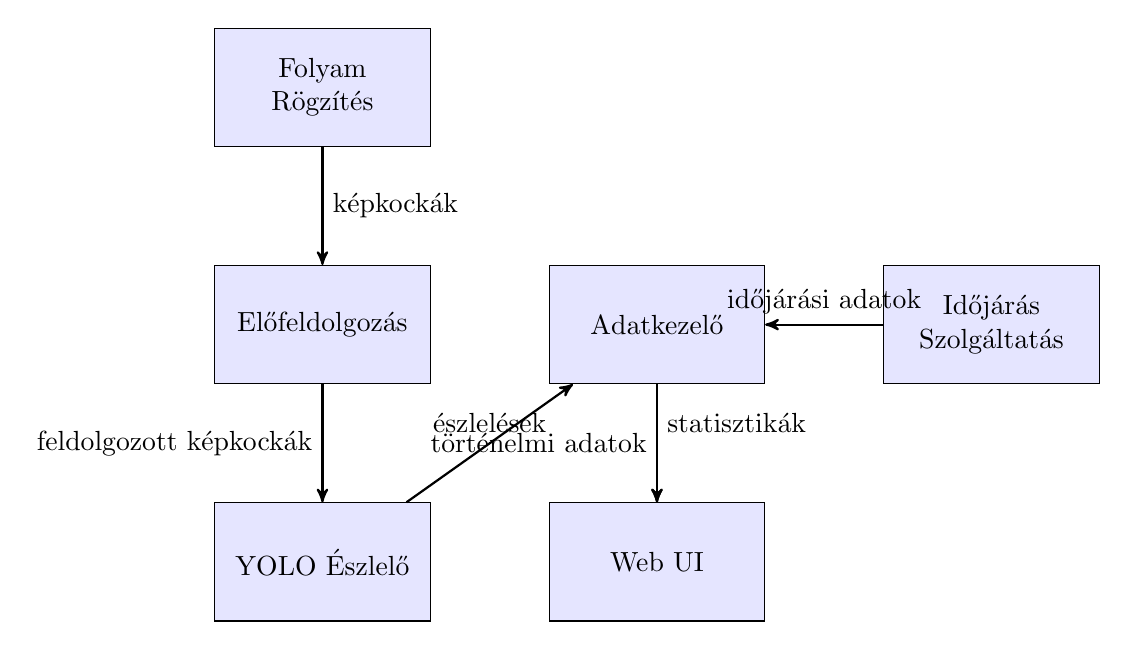
\begin{tikzpicture}[
node distance=1.5cm,
service/.style={
rectangle,
draw,
text width=2.5cm,
text centered,
minimum height=1.5cm,
fill=blue!10
},
arrow/.style={
->,
>=stealth',
thick
}
]
% Szolgáltatások
\node[service] (stream-capture) {Folyam Rögzítés};
\node[service, below=of stream-capture] (preprocessing) {Előfeldolgozás};
\node[service, below=of preprocessing] (yolo-detector) {YOLO Észlelő};
\node[service, right=of preprocessing] (data-manager) {Adatkezelő};
\node[service, below=of data-manager] (online-learner) {Online Tanuló};
\node[service, right=of data-manager] (weather-service) {Időjárás Szolgáltatás};
\node[service, right=of yolo-detector] (web-ui) {Web UI};

% Kapcsolatok
\draw[arrow] (stream-capture) -- (preprocessing) node[midway, right] {képkockák};
\draw[arrow] (preprocessing) -- (yolo-detector) node[midway, left] {feldolgozott képkockák};
\draw[arrow] (yolo-detector) -- (data-manager) node[midway, above] {észlelések};
\draw[arrow] (weather-service) -- (data-manager) node[midway, above] {időjárási adatok};
\draw[arrow] (data-manager) -- (online-learner) node[midway, left] {történelmi adatok};
\draw[arrow] (data-manager.south) -- (web-ui.north) node[midway, above right] {statisztikák};
\end{tikzpicture}
\caption{A Flowium rendszer mikro-szolgáltatásos architektúrája}
\end{figure}

\section{Konfiguráció}

Ebben a szakaszban ismertetésre kerül a rendszer konfigurációja. A Flowium rendszer beállításai főként környezeti változókkal történnek, amelyekhez egy \texttt{.env.example} nevű sablonfájl ad segítséget. Az alábbiakban felsorolásra kerülnek a legfontosabb változók:

\begin{itemize}
    \item \texttt{YOUTUBE\_URL}: A megfigyelt YouTube élő közvetítés URL-je.
    \item \texttt{LOCATION}, \texttt{LATITUDE}, \texttt{LONGITUDE}: Az időjárási szolgáltatás helyadatai.
    \item \texttt{CROP\_X}, \texttt{CROP\_Y}, \texttt{CROP\_WIDTH}, \texttt{CROP\_HEIGHT}: A videó kivágási régiójára vonatkozó koordináták.
\end{itemize}

\section{Telepítés és Üzemeltetés}

\subsection{Helyi Telepítés}

Ebben a részben bemutatásra kerül a rendszer helyi gépen történő telepítésének folyamata.

\subsubsection{Előfeltételek}

A rendszer futtatásához az alábbi szoftverekre van szükség:
\begin{itemize}
    \item Docker Engine
    \item Docker Compose
\end{itemize}

\subsubsection{Telepítési Lépések}

A telepítés az alábbi lépésekben történik:

\begin{enumerate}
    \item \textbf{Forrás fájlok kicsomagolása:} A projekt forráskódjának kibontása a zip fájlból, ami a docker fájlokat és a python kódokat tartalmazza.

    \item \textbf{Környezeti változók beállítása:} A \texttt{.env.example} fájl másolása és szerkesztése szükséges.
    \begin{lstlisting}[language=bash]
cp .env.example .env
nano .env
    \end{lstlisting}

    \item \textbf{Szolgáltatások építése és indítása:} A Docker Compose segítségével az összes konténer felépítése és indítása megtörténik.
    \begin{lstlisting}[language=bash]
docker-compose up -d --build
    \end{lstlisting}

    \item \textbf{Logok ellenőrzése:} A szolgáltatások működésének figyelése a következő paranccsal történhet:
    \begin{lstlisting}[language=bash]
docker-compose logs -f
    \end{lstlisting}

    \item \textbf{Web felület elérése:} A böngészőben a \url{http://localhost:8501} címen érhető el a Streamlit dashboard.
\end{enumerate}

\section{Továbbfejlesztési Lehetőségek és Kiegészítések}

\subsection{YOLO Modell Optimalizáció}

Ebben a részben bemutatásra kerül a YOLOv8 modell ONNX formátumra történő konvertálásának előnyei.

\subsubsection{ONNX Export}

Az ONNX (Open Neural Network Exchange) formátum használata jelentős teljesítménynövekedést eredményez CPU-alapú rendszereken. A projekt tartalmaz egy \texttt{export\_model.py} szkriptet, amely elvégzi a konverziót:

\begin{lstlisting}[language=bash, title=Modell konverzió]
python services/yolo-detector/export_model.py
\end{lstlisting}

\subsubsection{Teljesítmény Összehasonlítás}

\begin{table}[h]
\centering
\begin{tabular}{|l|l|l|}
\hline
\textbf{Formátum} & \textbf{Fájlméret} & \textbf{Inferencia idő (CPU)} \\
\hline
PyTorch (.pt) & 6.2 MB & \textasciitilde200 ms \\
ONNX (.onnx) & 12.2 MB & \textasciitilde80 ms \\
\hline
\end{tabular}
\caption{YOLO Modell Teljesítmény Összehasonlítás}
\end{table}

A táblázatból látható, hogy bár az ONNX fájl mérete közel kétszerese a PyTorch modellnek, a CPU-alapú inferencia sebessége több mint kétszeresére növekszik.

\subsection{Web UI Kiegészítések}

Ebben a részben bemutatásra kerülnek a webes felület funkciói.

\subsubsection{Analytics Tab - Legutóbbi Detekciók}

Az Analytics lapon megjelenik egy új szekció, amely valós időben jeleníti meg az utolsó 10 detekciót. A megjelenítés táblázatos formában történik, amely a következő oszlopokat tartalmazza:

\begin{itemize}
    \item Időpont (óra:perc:másodperc)
    \item Dátum (év-hónap-nap)
    \item Jármű típusa
    \item Konfidencia érték
    \item Detekció azonosító
\end{itemize}

\subsubsection{Predictions Tab}

Ebben a részben bemutatásra kerül a rendszer negyedik lapja, amely a gépi tanulással kapcsolatos funkciókat tartalmazza.

\paragraph{Modell Teljesítmény Mutatók:}

A lap tetején négy oszlopban jelennek meg a fő metrikák:
\begin{itemize}
    \item \textbf{Tanított minták száma:} Az eddigi betanítások összesített mennyisége
    \item \textbf{Mean Absolute Error (MAE):} A modell átlagos abszolút hibája
    \item \textbf{Modell státusz:} Ready (kész) vagy Training (tanulás alatt)
    \item \textbf{Átlagos hiba:} Járművek számában kifejezve
\end{itemize}

\paragraph{24 Órás Előrejelzés:}

Egy interaktív Plotly diagram jeleníti meg a következő 24 óra várható forgalmát. A diagram x tengelyén az idő, y tengelyén pedig a becsült járműszám látható.

\paragraph{Tanítási Történet:}

Az utolsó 20 tanítási minta megjelenítése történik egy kombinált line chart-on, amely összeveti az előrejelzett és a valós értékeket. Ez lehetővé teszi a modell pontosságának vizuális ellenőrzését.

\paragraph{Hiba Eloszlás:}

Egy hisztogram ábra mutatja a predikciós hibák eloszlását, amely segít megérteni, hogy a modell mennyire konzisztensen jósol.

\section{Képek a Web-es felületről}

\begin{figure}[H]
    \centering
    \includegraphics[width=\linewidth]{image/kep_4.png}
    \caption{Kép a folyamatról: bejövő videó, előfeldolgozás (vágás, fényerő, gamma, kontraszt), detektált kép}
    \label{fig:kep4}
\end{figure}

\begin{figure}[H]
    \centering
    \includegraphics[width=80pt]{image/kep_5.png}
    \caption{Feldolgozási sebesség}
    \label{fig:kep5}
\end{figure}

\begin{figure}[H]
    \centering
    \includegraphics[width=\linewidth]{image/kep_6.png}
    \caption{Teljes kép releváns része, kivágott terület}
    \label{fig:kep6}
\end{figure}

\begin{figure}[H]
    \centering
    \includegraphics[width=\linewidth]{image/kep_7.jpg}
    \caption{Feldolgozott kép}
    \label{fig:kep7}
\end{figure}

\end{document}
